\documentclass[10pt]{article}
\usepackage[utf8]{inputenc}
\usepackage{geometry} % to change the page dimensions
\geometry{a4paper}
\usepackage{authblk}

%% Packages
\usepackage{graphicx, subcaption}
\usepackage{amsmath,amssymb,amsthm,amsfonts}
\usepackage{bm}
\usepackage{algorithm, algorithmic}
\usepackage{multirow}
\usepackage{bbm}
\usepackage{hyperref,url}
\usepackage{kotex}
\usepackage[labelformat=simple]{subcaption}

\usepackage{tikz}
\usetikzlibrary{shapes.geometric, arrows, positioning, calc}
\usetikzlibrary{backgrounds}
\usetikzlibrary{arrows.meta}

\tikzstyle{title} = [rectangle, minimum width=3cm, minimum height=1cm, text centered, draw=black, text width=3cm, fill=white!100]
\tikzstyle{startstop} = [rectangle, rounded corners, minimum width=3cm, minimum height=1cm,text centered, draw=black, fill=red!30]
\tikzstyle{io} = [trapezium, trapezium left angle=70, trapezium right angle=110, minimum width=3cm, minimum height=1cm, text width=1.3cm, text centered, draw=black, fill=blue!30]
\tikzstyle{process} = [rectangle, minimum width=3cm, text width=3cm, minimum height=1cm, text centered, draw=black, fill=orange!30]
\tikzstyle{decision} = [diamond, minimum width=3cm, minimum height=1cm, text centered, draw=black, fill=green!30]
\tikzstyle{arrow} = [thick,->,>=stealth]

\captionsetup[figure]{labelsep=period}
% \renewcommand{\thefigure}{\Roman{figure}}
% \captionsetup[subfigure]{labelformat=parens} % default is 'parens'
% \renewcommand{\thesubfigure}{\thefigure.\alph{subfigure}.}
\renewcommand\thesubfigure{(\alph{subfigure})}

%% Theorems
\theoremstyle{plain}
\newtheorem{theorem}{Theorem}[section]
\newtheorem{proposition}[theorem]{Proposition}
\newtheorem{lemma}[theorem]{Lemma}

\theoremstyle{remark}
\newtheorem{remark}[theorem]{Remark}
\newtheorem{example}[theorem]{Example}

\theoremstyle{definition}
\newtheorem{definition}[theorem]{Definition}

%% Equations
\numberwithin{equation}{section}

%% Algorithms
\renewcommand\algorithmicdo{}
\renewcommand\algorithmicthen{}
\renewcommand\algorithmicendfor{\textbf{end}}

%% Macros
\def\chfun{\mathbbm{1}}
\def\skel{\mathcal{S}}
\def\calc{\mathcal{C}}
\def\sko{\hat{\mathcal{S}}}
\def\ske{\mathcal{S}^8}
\def\endske{E\left(\mathcal{S}^8\right)}
\def\endomc{E\left(\Omega_c\right)}


\def\gphi{\nabla\phi}
\def\ngphi{\left|\nabla\phi\right|}
\def\ngphii{\left|\nabla\phi_i\right|}
\def\fci{F_{c,\,i}}
\def\fcj{F_{c,\,j}}
\def\cm{\, ,}
\def\pd{\, .}

\def\omi{\Omega_i}
\def\oma{\Omega_a}
\def\ome{\Omega_E}
\def\oms{\Omega_S}
\def\omc{\overline{\Omega}_P}
\def\omcc{\Omega_P}
\def\ER{\Omega_{Er}}

\def\opp{\Omega_{\phi_i}^+}
\def\opn{\Omega_{\phi_i}^-}
% \def\opo{\Omega_{\phi}^0}
\def\opo{C_{\phi_i}}

\def\sdf{\mbox{SDF}}

\DeclareMathOperator*{\argmax}{arg\,max}
\DeclareMathOperator*{\argmin}{arg\,min}
% \def\tOmega{\tilde{\Omega}}
% \def\tGamma{\tilde{\Gamma}}
% \def\tV{\tilde{V}}
% \def\W{\mathbb{W}}
% \def\tu{\tilde{u}}
% \def\bu{\bar{u}}
% \def\hu{\hat{u}}
% \def\bl{\bar{\lambda}}
% \def\p{\mathbf{p}}
% \def\P{\mathbf{P}}
% \def\intO{\int_{\Omega}}
% \def\intOs{\int_{\Omega_s}}
% \def\m{\mathbf{m}}
% \def\n{\mathbf{n}}
% \def\blambda{\bm{\lambda}}

% \def\tE{\tilde{E}}
% \def\N{\mathcal{N}}

% \def\div{\mathrm{div}}
% \def\proj{\mathrm{proj}}
% \def\prox{\mathrm{prox}}
% \def\ran{\mathrm{ran}\,}
% \def\ed{\mathrm{ed}}
% \def\supp{\mathrm{supp}\,}
% \def\TOL{\mathrm{TOL}}
% \DeclareMathOperator*{\argmin}{\arg\min}

% Text Color and Strike
\usepackage[normalem]{ulem}
\usepackage{color}
\newcommand{\red}[1]{{\color{red}{#1}}}
\newcommand{\blue}[1]{{\color{blue}{#1}}}

\title{ Individual Tooth Segmentation in Human Teeth Images Using Pseudo Edge-Regions Obtained by Deep Neural Networks }
\author{Seongeun Kim and Chang-Ock Lee}
\affil{Department of Mathematical Sciences, KAIST, Daejeon 34141, Korea}
\date{ }

\begin{document}
\maketitle

\begin{abstract}
In human teeth images taken outside the oral cavity with a general digital camera, it is difficult to segment individual tooth due to common obstacles such as weak edges, intensity inhomogeneities and strong light reflections. In this work, we propose a method for segmenting individual tooth in human teeth images. The key of the method is to obtain pseudo edge-regions using deep neural networks. After obtaining landmarks for each tooth regions in the pseudo edge-region, we apply an active contour model to segment the individual tooth. We also present a strategy using existing model-based methods for labeling the data required for neural network training.
\end{abstract}

{\small \textbf{Key words}
Tooth segmentation, Neural network, Geometric attraction--driven flow, Edge-region, Light reflection}

{\small \textbf{AMS subject classifications}
94A08, 68T07}

%% Main text starts ---------------------------------------------------------------------------------------------------
% Section: Introduction
\section{Introduction}
\label{Sec:Introduction}

Image segmentation is one of major topics in the field of computer vision. The main goal of image segmentation is to segment objects in an image according to a specific purpose and many outstanding methodologies have been developed. The active contour model is one of the popular methods for the image segmentation. It makes the contour surrounding an object move to the boundary of the object with the designed force~\cite{Kass:1988:Snakes}; gradient vector flows~\cite{Xu:1997:GVF}, geodesic active contours~\cite{Caselles:1997:GAC} and balloon forces~\cite{Cohen:1991:Balloon} are well-known models with different forces. There are also variational models that uses statistical information of intensities in an image~\cite{Park:2014:SRM,Zhu:1996:RegCompet}. In \cite{Chan:2001:chanvese}, unlike the previous methods using edge maps, a region-based active contour method was proposed.

Segmentation of individual tooth in human teeth images has been mainly performed on computed tomography (CT) or X-ray images~\cite{Yuan:2020:teethParanomic,Naumovich:2015:teethCT3D,Said:2006:teethxray,Shah:2006:teethautoseg}. Teeth are easily segmented in these CT or X-ray images since the intensity of the teeth region is much stronger than the gums or tissues. However, segmenting individual tooth in a teeth image taken outside the oral cavity with a general digital camera is a more difficult problem. In the teeth images, not only weak edges and light reflections appear, but also colors and illuminance are inhomogeneous due to plaque and oral structure, which are major obstacles to segmentation of individual tooth. Several attempts have been made to segment individual tooth in teeth images. In~\cite{Na:2014LteethMorph} the watershed algorithm~\cite{Vincent:1991:watershed} with color information was proposed. In recent studies \cite{Kim:2020,Pham:2020,Zhu:2020:teethMaskrcnn}, segmentations using deep learning methods based on Mask R--CNN \cite{He:2018:MRCNN} were proposed. In~\cite{WU:2016}, a supervised learning method BEL~\cite{Dollar:2006:BEL} was used to obtain the individual tooth boundaries. Although the model-based method in~\cite{Na:2014LteethMorph} is reliable, it produces poor results when applied to images obtained in an unrefined environment. On the other hand, it is well known that supervised learning methods can give excellent results for a variety of images, but require sufficient amount of training data for stable performance, and that the labeling process of training data takes a lot of time and effort.

The main applications of individual tooth segmentation are reconstruction of 3D tooth models, postmortem identification of deceased persons, and dental healthcare. In particular, the 3D teeth model reconstruction was developed based on individual tooth segmentation in CT images~\cite{Yuan:2020:teethParanomic,Naumovich:2015:teethCT3D}. However, in a recent study~\cite{WU:2016}, a 3D teeth model reconstruction method using individual tooth boundaries in a single teeth image was proposed.

In this paper, we segment individual tooth regions using the deep neural network and active contour model. First, we obtain the pseudo edge-region using a deep neural network. When preparing data for training the networks, manually select regions on the tooth boundary among edge-regions acquired by geometric attraction-driven flow (GADF). After that, active contour model is applied to segment regions with initial contours obtained from the pseudo edge-region. Finally, by identifying tooth and non-tooth regions, only the tooth region is obtained as a result.

The remainder of this paper is organized as follows. In Section~\ref{Sec:er_teeth}, we will discuss geometric attraction-driven flow (GADF), edge-regions, and problems of edge-regions obtained from teeth images. In Section~\ref{Sec:PM}, the proposed algorithm is described, and the experimental results are presented in Section~\ref{Sec:result}. We will conclude this paper in Section~\ref{Sec:Conclusion}. 

% Sec:Background
\section{GADF, edge-regions and segmentations}
\label{Sec:er_teeth}
In this section, we briefly review the GADF and edge-region in~\cite{Hahn:2006,Hahn:2010:GADF}, which play key roles in segmenting individual tooth. Then we will show that the edge-regions obtained by GADF are incomplete due to the problematic features of the teeth image.

% Subsec:GADF
\subsection{GADF}
\label{Subsec:GADF}
Let $I\colon\Omega\subset\mathbf{R}^2\rightarrow[0,\,1]$ be a given smooth gray image. The image intensity changes rapidly on the boundary of objects in the image. Thus, a point $x\in\Omega$ is defined as an edge point if
\begin{align*}
    u_x''(0)=0\cm %label{Def:edge}
\end{align*}
where
\begin{align*}
    u_x(s) = I\left( x + s\frac{\nabla{I(x)}}{|\nabla{I(x)}|} \right)\pd
\end{align*}
In \cite{Hahn:2010:GADF}, the GADF is defined as
\begin{align}
    F_a(x) = \mbox{sgn}(\ell(x))\frac{\nabla I(x)}{\left|\nabla{I(x)}\right|},\quad \forall{x}\in\Omega\cm  \label{Def:gadf}
\end{align}
where $\mbox{sgn}$ is the sign function and 
\begin{align*}
    \ell(x) &= \int^{\epsilon}_{0} {u'_x(s)}\,ds - \int^{0}_{-\epsilon} {u'_x(s)}\,ds\quad\mbox{for a small}~\epsilon > 0\pd
\end{align*}
By the definition, $F_a(x)$ points along the line $x + s\frac{\nabla{I(x)}}{|\nabla{I(x)}|}$ towards the edge point. The GADF can be naturally extended to color images; see~\cite{Hahn:2006,Hahn:2010:GADF}. In this paper, we consider the GADF only for grayscale images. A grayscale image are obtained by averaging each channel of a given color image.

% Subsection: Edge-regions
\subsection{Edge-regions}
\label{Subsec:edge-regions}

The edge-region is roughly defined as the curve of thin regions containing most of object boundaries, regardless of the strength of edges. In~\cite{Hahn:2010:GADF}, $\ome$ is a region, called the candidate of edge-region, where $F_a$ faces each other, i.e. 
\begin{align*}
    \ome = \left\{ x\in\Omega \mid F_a(x^*) \cdot F_a(x) < 0 ~\mbox{and}~ x^*=x+F_a(x) \right\}\pd %\label{Def:pre_er}
\end{align*}
Since $F_a$ is defined using normalized gradient, it is independent of the strength of edges. Thus $\ome$ is a region that satisfies the rough definition of the edge-region. But in practice, $\ome$ is a candidate for edge-region, because it contains many regions that are not intersected with the boundaries of the object. Hence it is necessary to remove them as many as possible. In~\cite{Hahn:2006}, the removing is performed by analyzing image intensity and morphology of candidate for edge-regions.

In Figure~\ref{Fig:edge_regions}, we can see that $\ome$ is well formed only at the boundary of objects for the synthetic image, but there are a lot of regions not intersected to object boundaries in the practical images. In the last row, edge-regions of several images obtained by removing unnecessary regions from the candidate of edge-regions are presented. We will elaborate about these regions in Section~\ref{Subsec:light_reflection}.

% Figure: Weak edges in teeth image
% \begin{figure}
%     \centering
%     \begin{subfigure}{1\textwidth}
%         \centering
%         \includegraphics[width=10cm]{./Figures/Fig1_img.png}
%         \caption{A teeth image \cite{T001}}
%         \label{fig:1a}
%     \end{subfigure} 
%     \newline 
    
%     \vspace{1mm}
    
%     \begin{subfigure}{.165\textwidth}
%         \centering
%         \includegraphics[width=2.4cm]{./Figures/Fig1_img1.png}
%         \includegraphics[width=2.4cm]{./Figures/Fig1_img3.png}
%         \includegraphics[width=2.4cm]{./Figures/Fig1_img2.png}
%         \caption{}
%     \end{subfigure}
%     \begin{subfigure}{.165\textwidth}
%         \centering
%         \includegraphics[width=2.4cm]{./Figures/Fig1_sbl1.png}
%         \includegraphics[width=2.4cm]{./Figures/Fig1_sbl3.png}
%         \includegraphics[width=2.4cm]{./Figures/Fig1_sbl2.png}
%         \caption{Sobel}
%     \end{subfigure}
%     \begin{subfigure}{.165\textwidth}
%         \centering
%         \includegraphics[width=2.4cm]{./Figures/Fig1_cny1.png}
%         \includegraphics[width=2.4cm]{./Figures/Fig1_cny3.png}
%         \includegraphics[width=2.4cm]{./Figures/Fig1_cny2.png}
%         \caption{Canny}
%     \end{subfigure}
%     \begin{subfigure}{.165\textwidth}
%         \centering
%         \includegraphics[width=2.4cm]{./Figures/Fig1_er1.png}
%         \includegraphics[width=2.4cm]{./Figures/Fig1_er3.png}
%         \includegraphics[width=2.4cm]{./Figures/Fig1_er2.png}
%         \caption{$\oma$}
%         \label{Fig:1d}
%     \end{subfigure}
%     \caption{(a) A teeth image and (b) sub-images in the green boxes. (c--d) Results of Sobel and Canny edge detectors with automatically chosen thresholds by MATLAB. (e) $\oma$ from GADF. Weak edges appear at the boundary between teeth and gums, the boundary between two teeth with similar color and brightness, and the junction of boundaries. As shown in the results, GADF can detect tooth boundaries much better than the other methods while there are many unnecessary parts. }
%     \label{Fig:weak_edges}
% \end{figure}
\begin{figure}
    \centering
    \begin{subfigure}{1\textwidth}
        \centering
        \includegraphics[width=10cm]{./Figures/Fig1_img.png}
        \caption{A teeth image \cite{T001}}
        \label{fig:1a}
    \end{subfigure} 
    \newline 
    
    \vspace{1mm}
    
    \begin{subfigure}{.165\textwidth}
        \centering
        \includegraphics[width=2.4cm]{./Figures/Fig1_img1.png}
        \includegraphics[width=2.4cm]{./Figures/Fig1_img3.png}
        \includegraphics[width=2.4cm]{./Figures/Fig1_img2.png}
        \caption{}
    \end{subfigure}

    \caption{(a) A teeth image and (b) sub-images in the green boxes. (c--d) Results of Sobel and Canny edge detectors with automatically chosen thresholds by MATLAB. (e) $\oma$ from GADF. Weak edges appear at the boundary between teeth and gums, the boundary between two teeth with similar color and brightness, and the junction of boundaries. As shown in the results, GADF can detect tooth boundaries much better than the other methods while there are many unnecessary parts. }
    \label{Fig:edge_regions}
\end{figure}

% Subsection: Active Contour Model
\subsection{Active Contour Model}
\label{Subsec:active_contour}



The movement of the contour is performed by a force applied in the normal direction to the contour. Therefore, by defining the appropriate force, we can move the contour to reach the boundary of the object. This kind of methods are called geometric active contours methods \cite{Caselles:1997:GAC,Xu:2000:ParamGeoAC} and are widely used formulated as a level set method.

As an initial contour evolves forward to edges, these unnecessary parts hinder the movement of the contour. In fact, except for connected components of $\oma$ with closed shape, it can be easily removed or disregarded; the components with a small size or flat image intensities around them are easily removed \cite{Hahn:2006}. For the components that cannot form a closed shape, the evolving contour can intrude from the ends and disregard the component. The connected components with closed shape are mainly caused by a strong light reflection. They, like a barrier, block the movement of the contour and make it difficult to find the correct tooth boundary. As a result, presence of such light reflections is a major obstacle to individual tooth segmentation. The described contour evolution is shown in Figure~\ref{Fig:er_outside}.

% Figure: Edge regions outside the tooth boundaries
\begin{figure}
    \centering
    % First row
    \begin{subfigure}{.24\textwidth}
        \centering
        \includegraphics[height=2.8cm]{./Figures/Fig2_img.png}
        \caption{}
        \label{Fig:2a}
    \end{subfigure}
    \begin{subfigure}{.24\textwidth}
        \centering
        \includegraphics[height=2.8cm]{./Figures/Fig2_er.png}
        \caption{$\ome$}
        \label{Fig:2b}
    \end{subfigure}
    \begin{subfigure}{.24\textwidth}
        \centering
        \includegraphics[height=2.8cm]{./Figures/Fig2_reser.png}
        \caption{}
        \label{Fig:2c}
    \end{subfigure}\\
    \vspace{1mm}
    % First row
    \begin{subfigure}{.025\textwidth}
        \centering
        \caption*{\rotatebox[origin=c]{90}{\hspace{-4mm} (d) Left tooth}}
    \end{subfigure}
    \begin{subfigure}{.18\textwidth}
        \centering
        \includegraphics[height=2.4cm]{./Figures/Fig2_evolve_1/iter0.png}
    \end{subfigure}
    \begin{subfigure}{.18\textwidth}
        \centering
        \includegraphics[height=2.4cm]{./Figures/Fig2_evolve_1/iter150.png}
    \end{subfigure}
    \begin{subfigure}{.18\textwidth}
        \centering
        \includegraphics[height=2.4cm]{./Figures/Fig2_evolve_1/iter250.png}
    \end{subfigure}
    \begin{subfigure}{.18\textwidth}
        \centering
        \includegraphics[height=2.4cm]{./Figures/Fig2_evolve_1/iter300.png}
    \end{subfigure}
    \begin{subfigure}{.18\textwidth}
        \centering
        \includegraphics[height=2.4cm]{./Figures/Fig2_evolve_1/iter1000.png}
    \end{subfigure}\\
    \vspace{1mm}
    % Second row
    \begin{subfigure}{.025\textwidth}
        \centering
        \caption*{\rotatebox[origin=c]{90}{\hspace{-4mm} (e) Right tooth}}
    \end{subfigure}
    \begin{subfigure}{.18\textwidth}
        \centering
        \includegraphics[height=2.4cm]{./Figures/Fig2_evolve_2/iter0.png}
    \end{subfigure}
    \begin{subfigure}{.18\textwidth}
        \centering
        \includegraphics[height=2.4cm]{./Figures/Fig2_evolve_2/iter200.png}
    \end{subfigure}
    \begin{subfigure}{.18\textwidth}
        \centering
        \includegraphics[height=2.4cm]{./Figures/Fig2_evolve_2/iter350.png}
    \end{subfigure}
    \begin{subfigure}{.18\textwidth}
        \centering
        \includegraphics[height=2.4cm]{./Figures/Fig2_evolve_2/iter650.png}
    \end{subfigure}
    \begin{subfigure}{.18\textwidth}
        \centering
        \includegraphics[height=2.4cm]{./Figures/Fig2_evolve_2/iter1000.png}
    \end{subfigure}\\
    \vspace{1mm}
    % Third row
    \begin{subfigure}{.025\textwidth}
        \caption*{\rotatebox[origin=c]{90}{\hspace{-3mm} (f) Outside}}
    \end{subfigure}
    \begin{subfigure}{.18\textwidth}
        \centering
        \includegraphics[height=2.4cm]{./Figures/Fig2_evolve_3/iter0.png}
    \end{subfigure}
    \begin{subfigure}{.18\textwidth}
        \centering
        \includegraphics[height=2.4cm]{./Figures/Fig2_evolve_3/iter200.png}
    \end{subfigure}
    \begin{subfigure}{.18\textwidth}
        \centering
        \includegraphics[height=2.4cm]{./Figures/Fig2_evolve_3/iter350.png}
    \end{subfigure}
    \begin{subfigure}{.18\textwidth}
        \centering
        \includegraphics[height=2.4cm]{./Figures/Fig2_evolve_3/iter650.png}
    \end{subfigure}
    \begin{subfigure}{.18\textwidth}
        \centering
        \includegraphics[height=2.4cm]{./Figures/Fig2_evolve_3/iter1000.png}
    \end{subfigure}\\

    \caption{(a) Teeth image with light reflection. (c) Results obtained from (b) by removing unnecessary components and with dilated. (d--f) From left to right, the contour evolution over time by \eqref{Eq:gadf} is shown. The first column shows initial contours located at (d) the left tooth, (e) the right tooth, and (f) outside of teeth. Observe that the contours intrude into the components when it meets ends but are blocked when meets regions with closed shape. Especially in (d), the contour cannot extract the entire tooth boundary because of the closed shape component. }
    \label{Fig:er_outside}
\end{figure}

액티브 컨투어에 대한 설명

Under this setting, contour evolution using a level set formulation is proposed in \cite{Hahn:2010:GADF}:
\begin{align}
    \frac{\partial}{\partial{t}}\phi(x,\,t) &= \mu\kappa(\phi)\left|\nabla\phi\right| - \chi_{\oma}F_a\cdot\nabla\phi + \chi_{\Omega_b}F_b|\nabla\phi|\cm \label{Eq:gadf}\\
    \phi(x,\,0) &= \phi_0(x)\cm \nonumber
\end{align}
where $\mu$ is a constant, $\phi_0$ is the initial signed distance function (SDF), $\chi$ is a characteristic function of the set of subscription and $\oma$ is a region, called the candidate of edge-regions, where $F_a$ faces each other, i.e.,
\begin{align*}
    \Omega_a = \delta_{S}\left( \Omega_E \right)\cm %\label{Def:oma}
\end{align*}
where
\begin{align*}
    \Omega_E = \left\{ x\in\Omega \mid F_a(x^*) \cdot F_a(x) < 0 ~\mbox{and}~ x^*=x+F_a(x) \right\}\pd %\label{Def:pre_er}
\end{align*}
and $\delta_{S}(X)$ is a dilation of a set $X$ by a $3 \times 3$ square structuring element $S$ with origin at its center. Observe that the initial contour goes outward in $\Omega_b = \Omega\setminus\Omega_a$ by a balloon force $F_b$ and approaches the edge by $F_a$ once it reaches in $\Omega_a$.

%%%%%%%%%%%%%%%%%%%%%%%%%%%%%%%%%%%%%%%%%%%%%%%%%%%%%%%%%%%%%%%%%%
MMMMMMMMMMMMMMMMMMOOOOOOOOOOOOOOOOOOOOOOOOOOOOOOOOOOOOOVVVVVVVVVVVVVVVVVVVVVVVVVVVVVVVVVVVEEEEEEEEEEEEEEEEEEEEEEEEEEEEEEEEEEEEEEEEE!!!!!!!!!!!!!!!!!!!!!!!!!!!!!!!!!!!!!!
%%%%%%%%%%%%%%%%%%%%%%%%%%%%%%%%%%%%%%%%%%%%%%%%%%%%%%%%%%%%%%%%%%%%


% Subsection: Light reflections in the teeth image
\subsection{Light reflections in teeth images}
\label{Subsec:light_reflection}

There have been several studies to remove light reflections in a single image \cite{SpecRemoval:2018,SpecRemoval:2020,SpecRemoval:2016,SpecRemoval:2015}. In these works, an image was separated into a non-reflective image and a reflection map in the image domain. These methods are based on the intensity histogram or assumption of a dichromatic image model using color information of the reflective region. However, in the case of teeth images, the colors of the light reflection and the tooth surface are almost the same due to the characteristics of human teeth. For this reason, when these methods are actually applied, parts of the tooth surface is also removed along with the light reflection. 

Although there was an attempt to remove the light reflection in teeth images using a single layer perceptron \cite{LeeRemoval:2010}, there is a limitation that it cannot be applied to a wide range of images because the perceptron has an extremely simple structure and learning is processed with only one image.

The most problematic thing is that even if light reflection is removed from the teeth image, individual tooth cannot be segmented immediately. This is because there are a lot of unnecessary edges besides the light reflection. If each is simple, it does not interfere with the movement of the contour, but if they stick together forming a large bunch or enclosing a region, it hinders the movement of the contour and becomes an obstacle to detecting the boundary of the tooth. In addition, when light reflection appears on the tooth boundary, the edge collapses when the light reflection is removed, so that the boundary becomes undetectable. Therefore, we seek a way to directly obtain only the edge-region near the tooth boundary, regardless of stains, noise or light reflection of the image. For this, a supervised learning method with deep neural networks is considered.

% Section: Proposed Method
\section{Proposed Method}
\label{Sec:PM}
In this section, we describe the steps of the proposed individual tooth segmentation algorithm. It has the following four main steps and the whole process is shown in Figure~\ref{Fig:flowchart}:

\begin{itemize}
\setlength{\itemindent}{5mm}
    \item[STEP 1] Obtaining pseudo edge-regions from a neural network,
    \item[STEP 2] Refinement of the pseudo edge-region,
    \item[STEP 3] Segmentation using active contours with competing ballon forces,
    \item[STEP 4] Identification of tooth and non--tooth region.
\end{itemize}

% Figure: Algorithm flowchart
\begin{figure}
    \centering
    \begin{subfigure}[]{1\textwidth}
        % \centering
        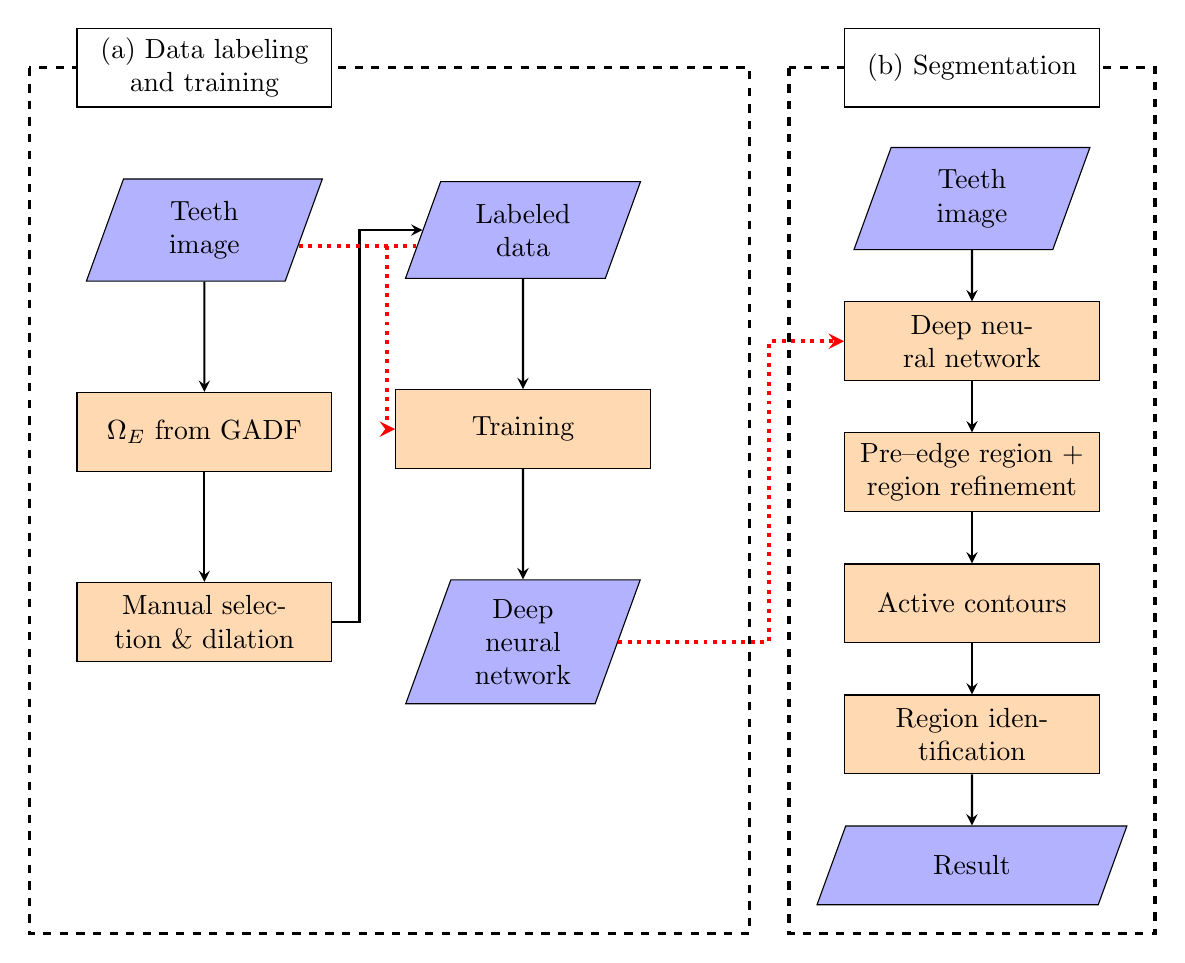
\begin{tikzpicture}[node distance=1.4cm and 1.5cm]
            \node (title1) [title] {(a) Data labeling and training};
            \node (title3) [title, right=6.5cm of title1] {(b) Segmentation};
            \node (teeth1) [io, below=.9cm of title1] {Teeth image};
            \node (pro11) [process, below=of teeth1] {$\Omega_E$ from GADF};
            \node (pro12) [process, below=of pro11] {Manual selection \& dilation};
            \node (label) [io, right=of teeth1] {Labeled data};
            \node (pro14) [process, below=of label] {Training};
            \node (dnn) [io, below=of pro14] {Deep neural network};
            
            \node (teeth3) [io, below=.5cm of title3] {Teeth image};
            \node (pro31) [process, below=.65cm of teeth3] {Deep neural network};
            \node (pro32) [process, below=.65cm of pro31] {Pre--edge region + region refinement};
            \node (pro33) [process, below=.65cm of pro32] {Active contours};
            \node (pro34) [process, below=.65cm of pro33] {Region identification};
            \node (res) [io, below=.65cm of pro34] {Result};
            
            \draw [arrow] (teeth1) -- (pro11);
            \draw [arrow] (pro11) -- (pro12);
            \draw [arrow] (pro12.east) -| ($(label.west) + (-.8, 0)$) -- (label.west);
            \draw [arrow] (label) -- (pro14);
            \draw [arrow] (pro14) -- (dnn);
            \draw [arrow] (teeth3) -- (pro31);
            \draw [arrow] (pro31) -- (pro32);
            \draw [arrow] (pro32) -- (pro33);
            \draw [arrow] (pro33) -- (pro34);
            \draw [arrow] (pro34) -- (res);

            \draw [red,line width=.5mm,dotted] ($(teeth1.east) + (-.07, -.2)$) |- ($(label.west) + (-.07, -.2)$);
            \draw [arrow, red,line width=.5mm, dotted] ($(label.west) + (-.45, -.2)$) |- (pro14.west);
            \draw [arrow, red,line width=.5mm, dotted] (dnn.east) -| ($(pro31.west) + (-.95,0)$) -- (pro31.west);
            \begin{scope}[on background layer]
                \draw[black,line width=.4mm,dashed] ($(title1.west)+(-.6,0)$)  rectangle ($(title1.east)+(5.3,-11)$);
                \draw[black,line width=.4mm,dashed] ($(title3.west)+(-.7,0)$)  rectangle ($(title3.east)+(.7,-11)$);
            \end{scope}
        \end{tikzpicture}
    \end{subfigure}
    \caption{Algorithm flowchart; (a) data labeling and training process (b) segmentation process.}
    \label{Fig:flowchart}
\end{figure}
    
% Subsection: Obtaining pre-edge regions from a neural network
\subsection{Obtaining pseudo edge-region from a neural network}
\label{Subsec:pre_er}

As shown in Figure~\ref{Fig:flowchart}(a), we make labels for training data using GADF and manual selection; first, we manually select the connected components of $\Omega_E$ intersecting the tooth boundary, then the label $Y\colon\Omega\subset\mathbf{R}^2\rightarrow\{0,\,1\}$ is defined as a binary image
\begin{align*}
    Y(x) =
    \begin{cases}
        1 & x\in\oms\cm\\
        0 & \mbox{otherwise}\cm
    \end{cases}
\end{align*}
where $\oms$ is obtained by dilating the selected regions from $\ome$ using an $\eta\times\eta$ square structuring element with the origin at its center. In Figure~\ref{Fig:labeling}, the labeling process is presented.

We consider a neural network consisting of the part of ResNeSt--50 \cite{Zhang:2020:ResNeSt} before the global average pooling layer as the encoder part and a custom upscaling module for the decoder part. The network takes a 3 channel image $X\colon\Omega\rightarrow\mathbf{R}^3$ as an input and produces an image $\hat{Y}\colon\Omega\rightarrow(0,\,1)$ as an output and is trained by minimizing the binary cross entropy (BCE) loss function \cite{Zhang:2018:BCE} of $Y$ and $\hat{Y}$. The entire network structure is shown in Figure~\ref{Fig:network}.

% Figure: Labeling images
\begin{figure}[]
    \centering
    \begin{subfigure}[]{.4\textwidth}
        \centering
        \includegraphics[height=3.8cm]{./Figures/Fig4_img.png}
        \caption{A training image \cite{T023}}
        \label{Fig:4a}
    \end{subfigure}
    \begin{subfigure}[]{.4\textwidth}
        \centering
        \includegraphics[height=3.8cm]{./Figures/Fig4_er.png}
        \caption{$\ome$}
        \label{Fig:4b}
    \end{subfigure}\\
    \vspace{1mm}
    \begin{subfigure}[]{.4\textwidth}
        \centering
        \includegraphics[height=3.8cm]{./Figures/Fig4_seler.png}
        \caption{Selected regions}
        \label{Fig:4c}
    \end{subfigure}
    \begin{subfigure}[]{.4\textwidth}
        \centering
        \includegraphics[height=3.8cm]{./Figures/Fig4_label.png}
        \caption{Labeled image $Y$}
        \label{Fig:4d}
    \end{subfigure}
    \caption{ Labeling process described in Section~\ref{Subsec:pre_er}: (a) An image in the training dataset. (b) The region $\Omega_E$. (c) Manually selected regions. (d) The labeled image obtained from (c) by the dilation. }
    \label{Fig:labeling}
\end{figure}

The network output $\hat{Y}(x)$ is the probability that an edge-region caused by the tooth boundary exists at $x$. We call
\begin{align}
    \omcc = \left\{ x\in\Omega \mid \hat{Y}(x) > 0.5 \right\} \label{Def:omcc}
\end{align}
as a pseudo edge-region of $X$, and examples of pseudo edge-regions for teeth images are shown in Figure~\ref{Fig:pre_er}.

% Figure: Network structure
\begin{subfigure}[]{1\textwidth}
    \newcommand*{\al}{0.3}%
    \newcommand*{\aw}{1.mm}%
    \newcommand*{\hei}{1.1 cm}%
    \newcommand*{\flr}{3.5cm}%
    \newcommand*{\wgap}{1cm}%
    \newcommand*{\init}{0}%
    \newcommand*{\wwa}{.2}%
    \newcommand*{\wwb}{.3}%
    \newcommand*{\wwc}{.4}%
    \newcommand*{\wwd}{.5}%
    \newcommand*{\wwe}{.6}%
    \newcommand*{\wwf}{.7}%
    \newcommand*{\wwg}{.9}%

    \newcommand*{\hha}{1}%
    \newcommand*{\hhb}{.9}%
    \newcommand*{\hhc}{.8}%
    \newcommand*{\hhd}{.6}%
    \newcommand*{\hhe}{.4}%
    \newcommand*{\hhf}{.2}%
    \newcommand*{\hhg}{.2}%
    \centering
    \begin{tikzpicture}[]
        \footnotesize
        \node (x0) at (0,0) [draw=none,minimum width=1mm,minimum height=\hei, fill=blue!50!white,label=above:{$3$}] {};
        \draw [-{Triangle[scale=.5]},line width=\aw,color=red!70!black] (x0.south) to ++(0,-\al);

        \node (x1) at ($(x0) + (0,-\hei-\al cm - .3 cm)$) [draw=none,minimum width=\wwa cm,minimum height=\hhb*\hei, fill=blue!50!white,label=above:{$32$}] {}; 
        \draw [-{Triangle[scale=.5]},line width=\aw,color=orange!80!white] (x1.east) -- ++(\al, 0);

        \node (x2) at ($(x1) + (\al+ \wwa/2 + \wwa/2,0)$) [draw=none,minimum width=\wwa cm,minimum height=\hhb*\hei, fill=blue!50!white,label=above:{$32$}] {};
        \draw [-{Triangle[scale=.5]},line width=\aw,color=orange!80!white] (x2.east) -- ++(\al, 0);
        
        \node (x3) at ($(x2) + (\al+\wwa/2 + \wwb/2,0)$) [draw=none,minimum width=\wwb cm,minimum height=\hhb*\hei, fill=blue!50!white,label=above:{$64$}] {};
        \draw [-{Triangle[scale=.5]},line width=\aw,color=yellow!80!black] (x3.south) to ++(0,-\al);
        
        \node (x4) at ($(x3) + (0,-\hhb*\hei-\al cm - .3 cm)$) [draw=none,minimum width=\wwb cm,minimum height=\hhc*\hei, fill=blue!50!white,label=above:{$64$}] {};
        \draw [-{Triangle[scale=.5]},line width=\aw,color=green!80!black] (x4.east) -- ++(\al, 0);
        
        \node (x5) at ($(x4) + (\al+\wwb/2 + \wwd/2,0)$) [draw=none,minimum width=\wwd cm,minimum height=\hhc*\hei, fill=blue!50!white,label=above:{$256$}] {};
        \draw [-{Triangle[scale=.5]},line width=\aw,color=green!80!black] (x5.east) -- node [above, color=black] {$\times 2$} ++(1.5*\al, 0);

        \node (x6) at ($(x5) + (1.5*\al+\wwd/2 + \wwd/2,0)$) [draw=none,minimum width=\wwd cm,minimum height=\hhc*\hei, fill=blue!50!white,label=above:{$256$}] {};
        \draw [-{Triangle[scale=.5]},line width=\aw,color=cyan!90!green] (x6.south) to  ++(0,-\al) {};

        \node (x7) at ($(x6) + (0,-\hhc*\hei-\al cm - .3 cm)$) [draw=none,minimum width=\wwe cm,minimum height=\hhd*\hei, fill=blue!50!white,label=above:{$512$}] {};
        \draw [-{Triangle[scale=.5]},line width=\aw,color=cyan!90!green] (x7.east) to node [above, color=black] {$\times 3$} ++(1.5*\al,0) {};

        \node (x8) at ($(x7) + (1.5*\al+\wwe/2 + \wwe/2,0)$) [draw=none,minimum width=\wwe cm,minimum height=\hhd*\hei, fill=blue!50!white,label=above:{$512$}] {};
        \draw [-{Triangle[scale=.5]},line width=\aw,color=blue!60!black] (x8.south) to  ++(0,-\al) {};

        \node (x9) at ($(x8) + (0,-\hhd*\hei-\al cm - .3 cm)$) [draw=none,minimum width=\wwf cm,minimum height=\hhe*\hei, fill=blue!50!white,label=above:{$1024$}] {};
        \draw [-{Triangle[scale=.5]},line width=\aw,color=blue!60!black] (x9.east) to node [above,color=black] {$\times 5$} ++(1.5*\al,0) {};

        \node (x10) at ($(x9) + (1.5*\al+\wwf/2 + \wwf/2,0)$) [draw=none,minimum width=\wwf cm,minimum height=\hhe*\hei, fill=blue!50!white,label=above:{$1024$}] {};
        \draw [-{Triangle[scale=.5]},line width=\aw,color=violet!90!black] (x10.south) to  ++(0,-\al) {};

        \node (x11) at ($(x10) + (0,-\hhe*\hei-\al cm - .3 cm)$) [draw=none,minimum width=\wwg cm,minimum height=\hhf*\hei, fill=blue!50!white,label=above:{$2048$}] {};
        \draw [-{Triangle[scale=.5]},line width=\aw,color=violet!90!black] (x11.east) to node [above, color=black] {$\times 2$} ++(1.5*\al,0) {};
        
        \node (x12) at ($(x11) + (1.5*\al+\wwg/2 + \wwg/2,0)$) [draw=none,minimum width=\wwg cm,minimum height=\hhf*\hei, fill=blue!50!white,label=above:{$2048$}] {};
        
        % latent variable
        \node (x13) at ($(x12) + (1.5*\al+\wwg/2 + \wwg/2,0)$) [draw=none,minimum width=\wwg cm,minimum height=2mm, fill=blue!50!white,label=above:{$2048$}] {};
        \draw [line width=\aw] (x12.east) to (x13.west) {};
        
        \node (x14) at ($(x13) + (0,\hhe*\hei+\al cm + .3 cm)$) [draw=none,minimum width=\wwg cm,minimum height=\hhe*\hei, fill=blue!50!white,label=above:{$2048$}] {};
        \draw [{Triangle[scale=.5]}-,line width=\aw,color=lime!50!black] (x14.south) to ++(0,-\al);
        
        \node (x15) at ($(x14) + (1.5*\al + \wwg/2 + \wwf/2,0)$) [draw=none,minimum width=\wwf cm,minimum height=\hhe*\hei, fill=blue!50!white,label=above:{$1024$}] {};
        \draw [-{Triangle[scale=.5]},line width=\aw,color=orange!80!white] (x14.east) to node [above, color=black] {$\times 2$} (x15.west) {};

        \node (x16) at ($(x15) + (0,\hhd*\hei+\al cm + .3 cm)$) [draw=none,minimum width=\wwf cm,minimum height=\hhd*\hei, fill=blue!50!white,label=above:{$1024$}] {};
        \draw [{Triangle[scale=.5]}-,line width=\aw,color=lime!50!black] (x16.south) to ++(0,-\al);
        
        \node (x17) at ($(x16) + (1.5*\al + \wwe/2 + \wwf/2,0)$) [draw=none,minimum width=\wwe cm,minimum height=\hhd*\hei, fill=blue!50!white,label=above:{$512$}] {};
        \draw [-{Triangle[scale=.5]},line width=\aw,color=orange!80!white] (x16.east) to node [above, color=black] {$\times 2$} (x17.west) {};

        \node (x18) at ($(x17) + (0,\hhc*\hei+\al cm + .3 cm)$) [draw=none,minimum width=\wwe cm,minimum height=\hhc*\hei, fill=blue!50!white,label=above:{$512$}] {};
        \draw [{Triangle[scale=.5]}-,line width=\aw,color=lime!50!black] (x18.south) to ++(0,-\al);
        
        \node (x19) at ($(x18) + (1.5*\al + \wwd/2 + \wwe/2,0)$) [draw=none,minimum width=\wwd cm,minimum height=\hhc*\hei, fill=blue!50!white,label=above:{$256$}] {};
        \draw [-{Triangle[scale=.5]},line width=\aw,color=orange!80!white] (x18.east) to node [above, color=black] {$\times 2$} (x19.west) {};

        \node (x20) at ($(x19) + (0,\hhb*\hei+\al cm + .3 cm)$) [draw=none,minimum width=\wwd cm,minimum height=\hhb*\hei, fill=blue!50!white,label=above:{$256$}] {};
        \draw [{Triangle[scale=.5]}-,line width=\aw,color=red!40!white] (x20.south) to ++(0,-\al);
        
        \node (x21) at ($(x20) + (1.5*\al + \wwd/2 + \wwc/2,0)$) [draw=none,minimum width=\wwc cm,minimum height=\hhb*\hei, fill=blue!50!white,label=above:{$128$}] {};
        \draw [-{Triangle[scale=.5]},line width=\aw,color=orange!80!white] (x20.east) to node [above, color=black] {$\times 2$} (x21.west) {};

        \node (x22) at ($(x21) + (0,\hei+\al cm + .3 cm)$) [draw=none,minimum width=\wwc cm,minimum height=\hei, fill=blue!50!white,label=above:{$128$}] {};
        \draw [{Triangle[scale=.5]}-,line width=\aw,color=red!40!white] (x22.south) to ++(0,-\al);
        
        \node (x23) at ($(x22) + (1.5*\al + \wwb/2 + \wwc/2,0)$) [draw=none,minimum width=\wwb cm,minimum height=\hei, fill=blue!50!white,label=above:{$64$}] {};
        \draw [-{Triangle[scale=.5]},line width=\aw,color=orange!80!white] (x22.east) to node [above, color=black] {$\times 2$} (x23.west) {};
        
        \node (x24) at ($(x23) + (\al + \wwb/2 + .1,0)$) [draw=none,minimum width=.1 cm,minimum height=\hei, fill=blue!50!white,label=above:{$1$}] {};
        \draw [-{Arc Barb[scale=.5]},line width=\aw,,color=red] (x23.east) to (x24.west) {};
    \end{tikzpicture}
    \caption{Network structure}
\end{subfigure}\\

\vspace{1mm}

\begin{subfigure}[]{.65\textwidth}
    \newcommand*{\hg}{.8}%
    \newcommand*{\wid}{.5}%
    \newcommand*{\hei}{1.3}%
    \newcommand*{\init}{0}%
    \newcommand*{\aw}{1mm}%
    \centering
    \begin{tikzpicture}
        \scriptsize
        \node (ipt) at (0,0) [rotate=90,draw=none,minimum width=\hei cm,minimum height=\wid cm, fill=orange!30!white, label=right:{$c$}, label={[xshift=-.7em, yshift=-.4em, rotate=90]}] {\footnotesize };
        
        \node (x1) at ($(ipt) + (\hg,0)$) [rotate=90,draw=none,minimum width=\hei cm,minimum height=\wid cm, fill=orange!30!white,  label=right:{$m$}, label={[xshift=-.7em, yshift=-.4em, rotate=90]}] {};

        \node (x21) at ($(x1) + (\hg,-1.5)$) [rotate=90,draw=none,minimum width=\hei cm,minimum height=\wid cm, fill=orange!30!white, label=right:{$m$}, label={[xshift=-.7em, yshift=-.4em, rotate=90]}] {};

        \node (x22) at ($(x1) + (\hg,1.5)$) [rotate=90,draw=none,minimum width=\hei cm,minimum height=\wid cm, fill=orange!30!white, label=right:{$m$}, label={[xshift=-.7em, yshift=-.4em, rotate=90]}] {};

        \node (sum1) at ($(x1) + (2*\hg,0)$) [circle, draw, very thick,minimum width=.1 cm,minimum height=.1 cm,text height=.15 cm, fill=none] {\footnotesize $+$};

        % \node (x3) at ($(x1) + (3*\hg,0)$) [rotate=90,draw=none,minimum width=\hei cm,minimum height=\wid cm, fill=orange!30!white, label=right:{$m$}, label={[xshift=-.7em, yshift=-.4em, rotate=90]}] {};

        \node (x4) at ($(x1) + (3*\hg,0)$) [rotate=90,draw=none,minimum width=.1 cm,minimum height=\wid cm, fill=orange!30!white, label=right:{$m$}, label={[xshift=-.7em, yshift=-.4em, rotate=90]}] {};

        \node (x5) at ($(x4) + (\hg,0)$) [rotate=90,draw=none,minimum width=.1 cm,minimum height=.7*\wid cm, fill=orange!30!white, label={[xshift=2.1em, yshift=.8em] $m/2$}, label={[xshift=-.7em, yshift=-.4em, rotate=90]}] {};

        \node (x61) at ($(x5) + (0,-.9)$) [rotate=90,draw=none,minimum width=.1 cm,minimum height=\wid cm, fill=orange!30!white, label=right:{$m$}, label={[xshift=-.7em, yshift=-.4em, rotate=90]}] {};

        \node (x62) at ($(x5) + (0,.9)$) [rotate=90,draw=none,minimum width=.1 cm,minimum height=\wid cm, fill=orange!30!white, label=right:{$m$}, label={[xshift=-.7em, yshift=-.4em, rotate=90]}] {};

        \node (prod11) at ($(x61) + (0,-1.1)$) [circle, draw, very thick,minimum width=.1 cm,minimum height=.1 cm, fill=none] {\footnotesize $\times$};
        \node (prod12) at ($(x62) + (0,1.1)$) [circle, draw, very thick,minimum width=.01 cm,minimum height=.01 cm,fill=none] {\scriptsize $\times$};

        \node (sum2) at ($(x5) + (\hg,0)$) [circle, draw, very thick,minimum width=.1 cm,minimum height=.1 cm,text height=.15 cm, fill=none] {\footnotesize $+$};

        \node (x7) at ($(x5) + (2*\hg,0)$) [rotate=90,draw=none,minimum width=\hei cm,minimum height=\wid cm, fill=orange!30!white, label=right:{$4m$}, label={[xshift=-.7em, yshift=-.4em, rotate=90]}] {};

        \node (sum3) at ($(x7) + (1*\hg,0)$) [circle, draw, very thick,minimum width=.1 cm,minimum height=.1 cm,text height=.15 cm, fill=none] {\footnotesize $+$};

        \node (x8) at ($(x7) + (2*\hg,0)$) [rotate=90,draw=none,minimum width=\hei cm,minimum height=\wid cm, fill=orange!30!white, label=right:{$4m$}, label={[xshift=-.7em, yshift=-.4em, rotate=90]}] {};

        \draw [-{Triangle[scale=.5]},line width=\aw,color=red] (ipt.south) to (x1.north) {};
        % \draw [-{Triangle[scale=.5]},line width=.2mm,color=black,dashed] (x1.south) to (x1.north) {};
        \draw [-{Triangle[scale=.5]},line width=\aw,color=orange!80!white] ($(x1.south) + (0,-.5)$) to (x21.north) {};
        \draw [-{Triangle[scale=.5]},line width=\aw,color=orange!80!white] ($(x1.south) + (0,.5)$) to (x22.north) {};
        % \draw [-{Triangle[scale=.5]},line width=\aw] (sum1.east) to (x3.north) {};
        \draw [-{Triangle[scale=.5]},line width=\aw] (sum1.east) to (x4.north) {};
        \draw [-{Triangle[scale=.5]},line width=\aw,color=magenta] (x4.south) to (x5.north) {};
        \draw [-{Bar[scale=.5]},line width=.5mm,color=magenta] (x5.west) to ++ (0,-.4);
        \draw [{Bar[scale=.5]}-,line width=.5mm,color=magenta] (x62.west) to ++ (0,-.4);
        \draw [-{Triangle[scale=.5]},line width=\aw,color=red] (sum2.east) to (x7);
        
        \draw [-{Triangle[scale=.5]},line width=.2mm] (x21.south) to (sum1) {};
        \draw [-{Triangle[scale=.5]},line width=.2mm] (x22.south) to (sum1) {};
        \draw [-{Triangle[scale=.5]},line width=.2mm] ($(x21.south) + (0,-.5)$) to (prod11);
        \draw [-{Triangle[scale=.5]},line width=.2mm] ($(x22.south) + (0,.5)$) to (prod12);
        \draw [{Triangle[scale=.5]}-,line width=.2mm] (prod11.north) to (x61.west);
        \draw [{Triangle[scale=.5]}-,line width=.2mm] (prod12.south) to ++(0,-.4);
        \draw [-{Triangle[scale=.5]},line width=.2mm] (prod11.east) to (sum2);
        \draw [-{Triangle[scale=.5]},line width=.2mm] (prod12.east) to (sum2);
        \draw [-{Triangle[scale=.5]},line width=.2mm] (prod12.east) to (sum2);
        \draw [-{Triangle[scale=.5]},line width=.2mm] (x7.south) to (sum3);
        \draw [dashed,line width=.25mm] (x1.west) -- ($(x21.west) + (0,-1cm)$) -- ($(x7.west) + (0,-2.5cm)$) -- (sum3.south) [-{Triangle[scale=.5]}];
        \draw [-{Triangle[scale=.5]},line width=.2mm] (sum3.east) to (x8.north);
    \end{tikzpicture}
    \caption{ResNeSt block with mid--channel size $m$ (RNS--$m$)}
\end{subfigure}
\begin{subfigure}[]{.3\textwidth}
    \newcommand*{\hg}{1.1}%
    \newcommand*{\wid}{.5}%
    \newcommand*{\hei}{2}%
    \newcommand*{\init}{-1}%
    \newcommand*{\aw}{.9mm}%
    \newcommand*{\al}{.5}%
    \centering
    \begin{tikzpicture}
        \footnotesize
        \matrix [draw,below left, thick] at (current bounding box) {
            \draw [line width=\aw,color=red!70!black] (\init,0) to ++(\al,0) node[right, color=black] {$3\times 3$ conv, $/2$, $+1$};\\

            \draw [line width=\aw,color=orange!80!white] (\init,0) to ++(\al,0) node[right, color=black] {$3\times 3$ conv, $+1$};\\

            \draw [line width=\aw,color=yellow!80!black] (\init,0) to ++(\al,0) node[right, color=black] {$3\times 3$ maxpool, $/2$, $+1$};\\

            \draw [line width=\aw,color=green!80!black] (\init,0) to ++(\al,0) node[right, color=black] {RNS--$64$};\\
            \draw [line width=\aw,color=cyan!90!green] (\init,0) to ++(\al,0) node[right, color=black] {RNS--$128$};\\
            \draw [line width=\aw,color=blue!60!black] (\init,0) to ++(\al,0) node[right, color=black] {RNS--$256$};\\
            \draw [line width=\aw,color=violet!90!black] (\init,0) to ++(\al,0) node[right, color=black] {RNS--$512$};\\

            \draw [line width=\aw] (\init,0) to ++(\al,0) node[right, color=black] {GAP};\\

            \draw [line width=\aw,color=lime!50!black] (\init,0) to ++(\al,0) node[right, color=black] {$2\times 2$, trans conv, $/2$};\\

            \draw [line width=\aw,color=red!40!white] (\init,0) to ++(\al,0) node[right, color=black] {Bilinear upscale};\\

            \draw [line width=\aw,color=red] (\init,0) to ++(\al,0) node[right, color=black] {$1\times 1$ conv};\\

            \draw [line width=\aw,color=magenta] (\init,0) to ++(\al,0) node[right, color=black] {Fully connected};\\
            \draw [-{Triangle[scale=.5]},line width=.3mm,color=black,dashed] (\init,0) to ++(\al,0) node[right, color=black] {Identity};\\

            \draw [-{Triangle[scale=.5]},line width=\aw,color=black] (\init,0) to ++(\al,0) node[right, color=black] {ReLU};
            \draw [-{Arc Barb[scale=.5]},line width=\aw,color=black] (-\init,0) to ++(\al,0) node[right, color=black] {Sigmoid};\\
            \draw [line width=\aw,color=black] (\init,0) to ++(\al,0) node[right, color=black] {None};
            \draw [-{Bar[scale=.5]},line width=\aw,color=black] (-\init,0) to ++(\al,0) node[right, color=black] {Softmax};\\
            \node (mod1) at (0,.25) [draw,minimum width=\init/2 cm,minimum height=.2 cm, fill=none] {\footnotesize MOD1} node[right, color=black] {$3 \times 3$ avgpool, $/2$, $+1$};\\
            \node (mod2) at (0,.25) [draw,minimum width=\init/2 cm,minimum height=.2 cm, fill=none] {\footnotesize MOD2} node[right, color=black] {$2 \times 2$ avgpool, $/2$, $+1$,};\\
            \node (mod22) at (0,.25) [draw=none,minimum width=\init/2 cm,minimum height=.2 cm, fill=none] {} node[right, color=black] {$1 \times 1$ conv, BN};\\
        };
    \end{tikzpicture}
\end{subfigure}

% Figure: pre_er
\begin{figure}[]
    \centering
    % \begin{subfigure}{.025\textwidth}
    %     \centering
    %     \caption*{\rotatebox[origin=c]{90}{\hspace{-4mm} (a) Input images}}
    %     \caption*{\rotatebox[origin=c]{90}{\hspace{-4mm} \footnotesize{(b) Pre--edge region} $\omcc$}}
    % \end{subfigure}
    \begin{subfigure}[]{.26\textwidth}
        \centering
        \includegraphics[height=2.4cm]{./Figures/Fig10_img0.pdf}
        \includegraphics[height=2.4cm]{./Figures/Fig10_neter0.pdf}
    \end{subfigure}
    \begin{subfigure}[]{.36\textwidth}
        \centering
        \includegraphics[height=2.4cm]{./Figures/Fig10_img1.pdf}
        \includegraphics[height=2.4cm]{./Figures/Fig10_neter1.pdf}
    \end{subfigure}
    \begin{subfigure}[]{.3\textwidth}
        \centering
        \includegraphics[height=2.4cm]{./Figures/Fig10_img5.pdf}
        \includegraphics[height=2.4cm]{./Figures/Fig10_neter5.pdf}
    \end{subfigure}
    \caption{First row: Input images. Second row: obtained pseudo edge-region from the neural network. }
    \label{Fig:pre_er}
\end{figure}

% Subsection: Refinement of pre--edge region
\subsection{Refinement of pseudo edge-region}
\label{Subsec:refine}

내용이바뀜내용이바뀜내용이바뀜내용이바뀜내용이바뀜내용이바뀜내용이바뀜내용이바뀜내용이바뀜내용이바뀜내용이바뀜내용이바뀜내용이바뀜

The region $\omcc$ in Section~\eqref{Def:omcc} is not yet perfect enough for segmenting individual tooth. Since it contains small fragments and leakages, which mean breakage of the closed curve, a refining process is applied to $\omcc$ to form a thick closed curve surrounding the individual tooth. First, small fragments and holes compared to the size of the image domain $\Omega$ are removed, and then dilation and erosion are sequentially applied by an $\omega \times\omega$ square structuring element with origin at its center. Second, since we want $\omcc$ to consist of thick closed curves,  Thus, we can fill the leakages by extending the ends of the curves in $\omcc$. By applying the chin--coding \cite{Freeman:1961:Chaincoding,Jonker:1992:Morphological} to the skeleton \cite{Blum:1967} of $\omcc$, we can find the parametric curves representing $\omcc$, see Figure~\ref{Fig:ex_ends_b}.

For each end, the strategy for extension is to return if not reached; if the leakage is not filled after a certain length of extension, then return and start extension in the next direction. Three directions are considered sequentially:
\begin{itemize}
    \setlength{\itemindent}{1.5mm}
    \item [(D--1)] If $\ome$ exists at the breaking of $\omcc$ and direction of $\ome$ coincides with the representative curve of $\omcc$, then $\omcc$ is extended along $\ome$,

    \item [(D--2)] Following the quadratic curve which is the least square quadratic approximation of the representative curve,

    \item [(D--3)] Following the straight line which is the least square linear approximation of the representative curve.
\end{itemize}
We call the resulting extension as $\omc$ and finally, we define a region $\ER := \omc\cap\ome$ which plays role of edge region. Examples of $\omc$ and $\ER$ are shown in Figure~\ref{Fig:ex_ends}.

% Figure: skeleton
\begin{figure}[]
    \centering
    \begin{subfigure}[]{.22\textwidth}
        \centering
        \includegraphics[height=3.5cm]{./Figures/Fig8_img.png}
        \caption{}
        \label{Fig:ex_ends_a}
    \end{subfigure}
    \begin{subfigure}[]{.22\textwidth}
        \centering
        \includegraphics[height=3.5cm]{./Figures/Fig8_curve.pdf}
        \caption{}
        \label{Fig:ex_ends_b}
    \end{subfigure}
    \begin{subfigure}[]{.22\textwidth}
        \centering
        \includegraphics[height=3.5cm]{./Figures/Fig8_ext.png}
        \caption{}
        \label{Fig:ex_ends_d}
    \end{subfigure}
    \begin{subfigure}[]{.22\textwidth}
        \centering
        \includegraphics[height=3.5cm]{./Figures/Fig8_use_er.png}
        \caption{$\ER$}
        \label{Fig:ex_useer_d}
    \end{subfigure}
    \caption{The process of extension from the ends of curves. (b) The parametric curves with ends (blue dots) are presented in $\omcc$ of the teeth image (a). (c) The extended region $\omc$. (d) Among $\ome$, the region $\ER$ is displayed in red. }
    \label{Fig:ex_ends}
\end{figure}

% Subsection: Segmentation using active contours with competing ballon forces
\subsection{Segmentation using active contours}
\label{Subsec:SegLevelset}

In this section, we denote $\sdf(A)$ by a SDF which is negative on the set $A$ and constantly zero on $\partial A$. In addition, for a SDF $\phi$, $\opp$, $\opn$ and $\opo$ denote the sets $\left\{x\mid \phi > 0 \right\}$, $\left\{x\mid \phi < 0 \right\}$ and $\left\{x\mid \phi = 0 \right\}$, respectively.

The movement of the contour is performed by a force applied in the normal direction to the contour. Therefore, by defining the appropriate force, we can move the contour to reach the boundary of the object. This kind of methods are called geometric active contours methods \cite{Caselles:1997:GAC,Xu:2000:ParamGeoAC} and are widely used formulated as a level set method. In this paper, we segment each tooth region using multiple active contours formulated as multiple level sets. Let $\{\Omega_i\}_{i=1}^N$ be a collection of all connected component of $\Omega\setminus\omc$. As shown in Figure~\ref{Fig:ex_ends_d}, $\omi$ is included in an individual tooth region, gum or oral cavity. Thus, to find a curve enclosing an individual tooth, we take the curve on $\partial\omi$ and push it outward until it reaches the boundary of the tooth. For this, we propose a contour evolution with a level set formulation:
\begin{align}
    \frac{\partial}{\partial{t}}\phi_i(x,\,t) &= \mu\kappa(\phi_i)\ngphii + \left( \chi_{\Omega\setminus\ER}\fci +\chi_{\omc\setminus\ER}F_s \right) \ngphii-\chi_{\ER}F_a\cdot \gphi \cm \label{Eq:proposed}\\
    \phi_i(x,\,0) &= \phi_{i,\,0}(x)\cm \nonumber
\end{align}
where $\mu$ is a constant, $\kappa(\phi)_i$ is the curvature of $\phi_i$, and $\phi_{i,\,0}(x)=\sdf(\omi)$ for all $i=1\cm\ldots\cm N$. Here are three forces $F_a$, $F_s$ and $\fci$; $F_a$ is GADF defined in~\eqref{Def:gadf}, $F_s$ is the statistically reinstating force proposed in~\cite{Park:2014:SRM}. The force $F_s(x)$ examines intensity distributions of in and out regions of a given contour and decided as $1$ or $-1$ to push the contour so that $x$ belongs to a region with more similar intensity. The force $\fci$ is the competing balloon force defined as
\begin{align*}
    \fci(x,\,t) =
        -1 - \sum_{j\neq i}\min\left(\phi_j(x,\,t) - 1,\,0\right)\cm\quad\forall i=1,\,\ldots,\,N\cm
\end{align*}
which is designed to inflate the set $\opn$ until it meets $\Omega_{\phi_{j}}^-$ for any $j\neq i$ and then stop.

Suppose that an initial contour $\opo$ is evolving by \eqref{Eq:proposed}. Basically, $\opn$ is inflated by $\fci$ so that $\opo$ enters the interior of the region $\omc$. In $\omc$, we consider three cases of $\opo$ in order: inside $\ER$, outside $\ER$ a way from other contours, and outside $\ER$ facing other contours. If $\opo$ is in $\ER$, it follows $F_a$ to the edge . If not, $\opo$ evolves by $\fci + F_s$ and edge is determined by the value of $F_s$ since $\fci$ only can have a value in $[-1,\,0]$. In the case that there are neither $\ER$ nor edges detected by $F_s$, the contour $\opo$ continues to evolve only with $\fci$ going until it encounters some other contours and determines an edge by competing each other.

% Subsection: Teeth and non-teeth region classification
\subsection{Identification of tooth and non-tooth regions}
\label{Subsec:regClass}

As a final step, the identification of the segmented regions remains. Since our goal is to segment each individual tooth from the result in Section~\ref{Subsec:SegLevelset}, we need to identify tooth and non-tooth regions. In a human teeth image, tooth and non-tooth regions can be easily distinguished by shape and color. Teeth are relatively white and convex in shape, thus non-tooth regions can be easily removed. We can check the shape or color of a region by considering several aspects: inertia tensor, curvature on the boundaries, and point distribution in a color space. The region having the following features is identified as a non--teeth region in order.

어펜딕스 가져오자어펜딕스 가져오자어펜딕스 가져오자어펜딕스 가져오자어펜딕스 가져오자어펜딕스 가져오자

% Section: Experimental results
\section{Experimental results and numerical aspect}
\label{Sec:result}

\textbf{Common parameters.} In all experiments, the parameter $\mu$ in~\eqref{} is fixed at $\mu=1$. In Section~\ref{}, $\eta=\lfloor|\Omega| / 600 + 1/2\rfloor$ and in Section~\ref{}, $\omega=2\lfloor\theta + 1/2\rfloor + 1$, where $\theta$ is the average thickness of $\omcc$ measured by sampling random points in $\omcc$. Also in Section~\ref{Subsec:refine}, small fragments with a skeleton shorter than $\sqrt{m^2+n^2} / 10$ and holes with size less than $mn / 10000$ are removed for an $m\times n$ image.

\noindent\textbf{Numerical schemes.} Overall, the finite difference scheme is applied to all derivatives. For the contour evolution \eqref{Eq:proposed}, the explicit Euler method is used. While performing the contour evolution, the level set function is frequently reinitialized by the method in \cite{SUSSMAN:1994}. The skeleton of $\omcc$ \eqref{} is obtained by applying a skeletonization algorithm of \cite{Zhang:1984} to $\left\{x \mid |\gphi(x)| < \sqrt{2}/2\right\}$ with $\phi=\sdf(\omcc)$.

\noindent\textbf{Data augmentation.} To get more diverse training data, data augmentation is applied. In each epoch, images are resized with randomly sampled height in $[256,\, 512]$, and $256\times256$ patch or its horizontal flip is randomly cropped \cite{He:2015:ResNet,Krizhevsky:2012:ImageNet}. Furthermore, for each image, the augmentation in the following list is randomly applied with a probability of $0.5$ within the given ranges:
\begin{itemize}
    \item Gaussian smoothing with $\sigma\in[0.25,\,0.75]$,
    \item Adding Gaussian noise with $\sigma\in[0.005,\,0.015]$,
    \item Gamma correction with $\gamma\in[0.5,\,2]$,
\end{itemize}

\noindent\textbf{Training data.} The training dataset consists of $46$ images obtained from web searches using various search terms. All teeth images contain \cite{} light reflections on the surface of teeth, gums or other parts.

\noindent\textbf{Training.} The neural network is trained by minimizing the BCE loss function \cite{Zhang:2018:BCE} using the Adam optimizer \cite{Kingma:2017}. The exponential decay rates for the moment of Adam optimizer are set $(\beta_1,\,\beta_2)=(0.9,\,0.999)$ and the learning rate is $0.005$. Network is trained over $10{,}000$ epochs with $46$ iterations for each epoch, and the parameters after the last epoch are selected. 

\noindent\textbf{Results.} In Figure~\ref{Fig:results}, several teeth images with its segmentation results for existing and proposed methods are presented. As shown in the figure, the proposed method shows prominent results. Quantitative measurement is impossible since there is no ground truth, but compared to the results of the existing methods, it can be seen that the tooth regions are neatly segmented. In particular, only the tooth regions are segmented in the teeth images the lips and the face part exist.

% Figure: Edge region candidate and results
\begin{figure}[]
    \newcommand*{\wdth}{2.5}%
    \newcommand*{\twdth}{.16}%
    \centering
    \begin{subfigure}[]{\twdth \textwidth}
        \centering
        \includegraphics[width=\wdth cm]{./Figures/Fig10_img0.pdf}
        \includegraphics[width=\wdth cm]{./Figures/Fig10_img1.pdf}
        \includegraphics[width=\wdth cm]{./Figures/Fig10_img5.pdf}
        \includegraphics[width=\wdth cm]{./Figures/Fig10_img8.pdf}
        \includegraphics[width=\wdth cm]{./Figures/Fig10_img18.pdf}
        \includegraphics[width=\wdth cm]{./Figures/Fig10_img17.pdf}
        \caption{Input images}
    \end{subfigure}
    \begin{subfigure}[]{\twdth \textwidth}
        \centering
        \includegraphics[width=\wdth cm]{./Figures/lee2010_0.pdf}
        \includegraphics[width=\wdth cm]{./Figures/lee2010_1.pdf}
        \includegraphics[width=\wdth cm]{./Figures/lee2010_5.pdf}
        \includegraphics[width=\wdth cm]{./Figures/lee2010_8.pdf}
        \includegraphics[width=\wdth cm]{./Figures/lee2010_18.pdf}
        \includegraphics[width=\wdth cm]{./Figures/lee2010_17.pdf}
        \caption{MCWA \cite{LeeWater:2010}}
        \label{Fig:lee2010}
    \end{subfigure}
    \begin{subfigure}[]{\twdth \textwidth}
        \centering
        \includegraphics[width=\wdth cm]{./Figures/lee2010s_0.pdf}
        \includegraphics[width=\wdth cm]{./Figures/lee2010s_1.pdf}
        \includegraphics[width=\wdth cm]{./Figures/lee2010s_5.pdf}
        \includegraphics[width=\wdth cm]{./Figures/lee2010s_8.pdf}
        \includegraphics[width=\wdth cm]{./Figures/lee2010s_18.pdf}
        \includegraphics[width=\wdth cm]{./Figures/lee2010s_17.pdf}
        \caption{MCWA2 \cite{LeeSegRemoval:2010}}
        \label{Fig:lee2010_2}
    \end{subfigure}
    \begin{subfigure}[]{\twdth \textwidth}
        \centering
        \includegraphics[width=\wdth cm]{./Figures/na2014_0.pdf}
        \includegraphics[width=\wdth cm]{./Figures/na2014_1.pdf}
        \includegraphics[width=\wdth cm]{./Figures/na2014_5.pdf}
        \includegraphics[width=\wdth cm]{./Figures/na2014_8.pdf}
        \includegraphics[width=\wdth cm]{./Figures/na2014_18.pdf}
        \includegraphics[width=\wdth cm]{./Figures/na2014_17.pdf}
        \caption{MWA \cite{Na:2014LteethMorph}}
        \label{Fig:na2014}
    \end{subfigure}
    \begin{subfigure}[]{\twdth \textwidth}
        \centering
        \includegraphics[width=\wdth cm]{./Figures/Fig10_res0.pdf}
        \includegraphics[width=\wdth cm]{./Figures/Fig10_res1.pdf}
        \includegraphics[width=\wdth cm]{./Figures/Fig10_res5.pdf}
        \includegraphics[width=\wdth cm]{./Figures/Fig10_res8.pdf}
        \includegraphics[width=\wdth cm]{./Figures/Fig10_res18.pdf}
        \includegraphics[width=\wdth cm]{./Figures/Fig10_res17.pdf}
        \caption{Our algorithm}
        \label{Fig:result}
    \end{subfigure}
    \caption{ Segmented results of several methods for input images \cite{T000,T008,T005,T018,T017}. }
    \label{Fig:results}
\end{figure}

% Section: Conclusion
\section{Conclusion}
\label{Sec:Conclusion}

In this paper, we proposed a method for individual tooth segmentation in a human teeth image. Including the strong light reflection, there are several obstacles that hinder the segmentation process. We solved these problem by acquiring pseudo edge-region using a deep neural network with supervised learning. In the labeling process, model-based methods were used to reduce time consumption and cost. In addition, we proposed contour evolution to inflating the initial contour using different forces depending on the situation 

to find the boundary of the tooth from te refined pseudo edge-regions + identification of tooth and non-tooth region. 

Among the existing methods, model-based methods show insufficient performance. Although the supervised learning method using Mask R--CNN has similar performance to ours, it is difficult to label the data for training. This work is significant in that it proposed an algorithm that can easily prepare training data while performing well through a combination of model-based methods and a supervised learning method. It is noted that the combination of the two methods produced a synergistic effect; model-based methods streamline the labeling process for training deep neural networks and the networks simplify the problem by inferring pseudo edge-regions. 

One of the most important application of individual tooth segmentation is the 3D teeth model reconstruction. That this study will be of great help in reconstructing a more sophisticated 3D teeth model from a 2D teeth image.

% Section: Acknowledgement
% \section*{Acknowledgement}

%% Appendix
\appendix
\section{List of features of non-tooth region}
\label{App:list_nonteeth}

The methods in the list below is applied sequentially for identification of tooth and non-tooth regions. For a region, let $c$ be the center of mass and $\mathcal{I}$ the inertia tensor about $c$. Then the inertia tensor has two eigenvalues $\Lambda$ and $\lambda$ ($\Lambda \le \lambda$). Let $v$ be an normalized eigenvector corresponding to the $\lambda$. Let the image $I$ be embedded into the CIELAB color space~\cite{} and denoted by $I_{LAB}(x)=[L(x),\,A(x),\,B(x)]$, and let $x^*\in\Omega$ be a point such that
\begin{align*}
    x^* = \argmax A(x)\pd
\end{align*}

\begin{itemize}
    \item [(F--1)] If the center of mass $c$ is outside the region, a region identified as a non-tooth region.

    \item [(F--2)] If the ratio $\Lambda / \lambda$ is larger than the average of the ratio for all regions and $|v\cdot e_1| \le \cos(\pi/4)$ for $e_1 = (1,\,0)$, the region identified as a non-tooth region.
    
    \item [(F--3)] Count the number of points with positive or negative curvature on the boundary of region. If there are more points of negative curvature than points of positive curvature, the region is identified as a non-tooth region
    
    \item [(F--4)] For each vertical line passing through the region, values of $I_{LAB}$ on the points where the line passes are clustered together $I_{LAB}(x^*)$ by the $k$--means clurstering algorithm.
\end{itemize}

%% References
\bibliographystyle{siam}
\bibliography{bibliography}

\end{document}
